\section{Coast and Burn}
The principle of the coast and burn functionality is described in this section.
Coast and burn, also known as pulse and glide, is a fuel saving method. It consists of rapidly accelerating (pulse) to a given speed by utilizing the engine at its peak effectiveness. Followed by this is a period of coasting (glide) down to a set speed. The burn-coast sequence is then repeated around two specified velocities to achieve the highest possible fuel efficiency.

Usually one would think that the coast and burn method would consume more fuel than the method of applying a constant current over a period of time to maintain a particular speed. However, this assumption is incorrect. By applying a high current to an engine for a short period instead of a constant current, one achieves a considerably better fuel economy. This can be explained by an engine’s efficiency rate. An engine performs a lot better when it is under a high load. This supports the fact that when one accelerates rapidly to a specified velocity the engine is subjected to a high load, however when subjecting the engine to a constant acceleration the engine will not be subjected to a high load thus not being as efficient as it could be.

In AU2 this principle is utilized to its fullest potential. A rundown of what happens in the motor controller is as follows: when the car is turned on, it will start accelerating rapidly. When it reaches a given velocity, it will start coasting, meaning the motor will shutdown. Then it will proceed to slow down until it reaches a specified speed before starting to accelerate again. This process will keep on repeating until either there is an overcurrent on the engine or the driver presses a button to disable the coast and burn functionality.

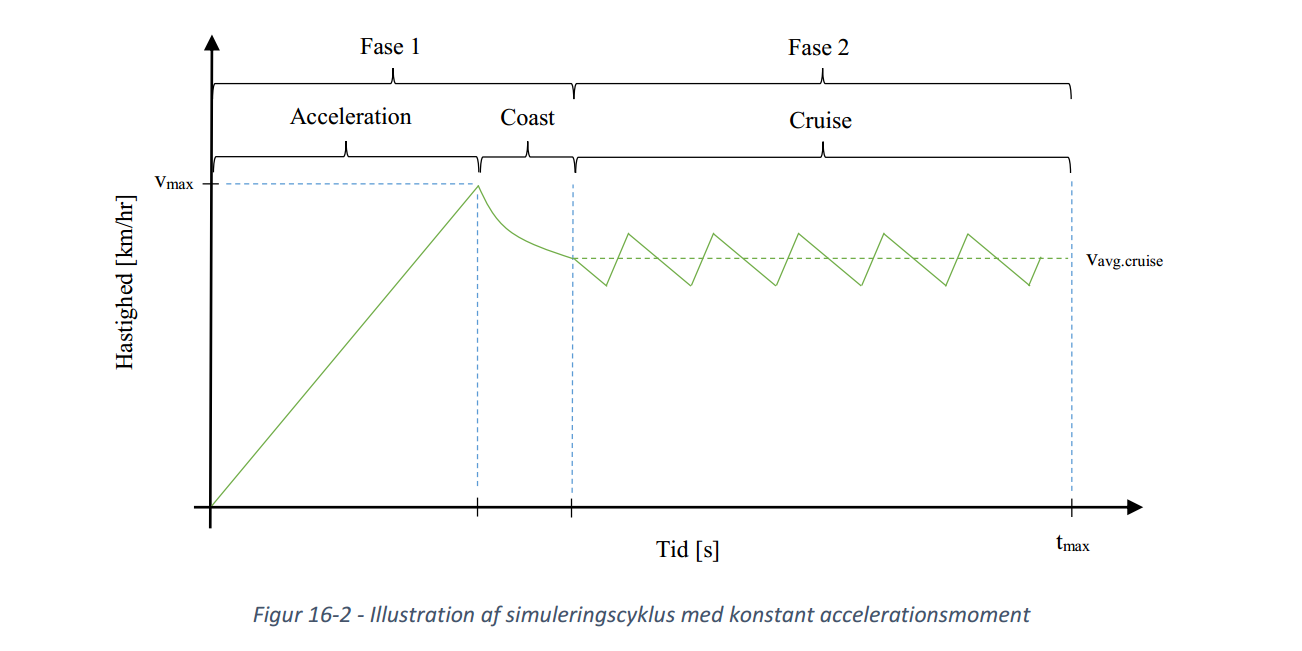
\includegraphics[width=1.0\linewidth]{Software/Coastburn.PNG}

\fxnote{Reference til drivlinje rapporten}

